\documentclass[11pt,a4paper]{article}

% packages
\usepackage[utf8]{inputenc}
\usepackage{amsmath}
\usepackage[T1]{fontenc}
\usepackage{setspace}
\usepackage{enumitem}
\usepackage{amsmath}
\usepackage{booktabs}
\usepackage{fullpage} 
\usepackage{tabularx}
\usepackage{amssymb, amstext, amsmath}
\usepackage{fancyhdr}
\usepackage{graphicx}
\usepackage{algorithmic}
\usepackage[ruled,vlined]{algorithm2e}
\usepackage{url}
\usepackage[bookmarks,unicode=true,pdftex,a4paper]{hyperref}
\usepackage[round]{natbib}
\usepackage[usenames,dvipsnames]{color, xcolor}
\headsep1cm

% macros
% misc
\newcommand\todo[1]{\textcolor{red}{TODO: #1}}
\newcommand\hide[1]{\textcolor{white}{#1}}

% formatting
\newcommand\bld[1]{\textbf{#1}}
\newcommand\ul[1]{\underline{#1}}
\newcommand\n[1]{\numprint{#1}}
\newcommand{\ts}{\textsuperscript}
\newcommand\red[1]{\textcolor{red}{#1}}
\newcommand\blue[1]{\textcolor{blue}{#1}}
\newcommand\link[2]{\href{#1}{\textcolor{blue}{\underline{#2}}}}

% sets
\newcommand\set[1]{\mathcal{#1}}
\newcommand\bb[1]{\mathbb{#1}}
\renewcommand\:{\colon} % for use with \sset, etc.
\newcommand{\sset}[1]{\left\{\,#1\,\right\}} % { ? }, automatic brackets
\newcommand{\ssets}[1]{\left\{#1\right\}} % {?}, automatic brackets
\newcommand{\ssetn}[1]{\{\,#1\,\}} % { ? }, normal brackets

% table formatting
% To better align bold entries in S columns (still broken)
% \usepackage{siunitx}
% \robustify\bfseries
% \newrobustcmd{\bfcell}{\bfseries}

% vector variables (taken from macros by Rainer Gemulla)
\newcommand\vect[1]{{\boldsymbol{#1}}}
\newcommand\va{\vect{a}}
\newcommand\vb{\vect{b}}
\newcommand\vc{\vect{c}}
\newcommand\vd{\vect{d}}
\newcommand\ve{\vect{e}}
\newcommand\vf{\vect{f}}
\newcommand\vg{\vect{g}}
\newcommand\vh{\vect{h}}
\newcommand\vi{\vect{i}}
\newcommand\vj{\vect{j}}
\newcommand\vk{\vect{k}}
\newcommand\vl{\vect{l}}
\newcommand\vm{\vect{m}}
\newcommand\vn{\vect{n}}
\newcommand\vo{\vect{o}}
\newcommand\vp{\vect{p}}
\newcommand\vq{\vect{q}}
\newcommand\vr{\vect{r}}
\newcommand\vs{\vect{s}}
\newcommand\vt{\vect{t}}
\newcommand\vu{\vect{u}}
\newcommand\vv{\vect{v}}
\newcommand\vw{\vect{w}}
\newcommand\vx{\vect{x}}
\newcommand\vy{\vect{y}}
\newcommand\vz{\vect{z}}
\newcommand\vzero{\vect{0}}
\newcommand\vone{\vect{1}}

\newcommand\valpha{\vect{\alpha}}
\newcommand\vbeta{\vect{\beta}}
\newcommand\veps{\vect{\epsilon}}
\newcommand\vdelta{\vect{\delta}}
\newcommand\vtheta{\vect{\theta}}
\newcommand\vsigma{\vect{\sigma}}
\newcommand\vpi{\vect{\pi}}
\newcommand\vlambda{\vect{\lambda}}

% matrix variables (taken from macros by Rainer Gemulla)
\newcommand\mA{\vect{A}}
\newcommand\mB{\vect{B}}
\newcommand\mC{\vect{C}}
\newcommand\mD{\vect{D}}
\newcommand\mE{\vect{E}}
\newcommand\mF{\vect{F}}
\newcommand\mG{\vect{G}}
\newcommand\mH{\vect{H}}
\newcommand\mI{\vect{I}}
\newcommand\mJ{\vect{J}}
\newcommand\mK{\vect{K}}
\newcommand\mL{\vect{L}}
\newcommand\mM{\vect{M}}
\newcommand\mN{\vect{N}}
\newcommand\mO{\vect{O}}
\newcommand\mP{\vect{P}}
\newcommand\mQ{\vect{Q}}
\newcommand\mR{\vect{R}}
\newcommand\mS{\vect{S}}
\newcommand\mT{\vect{T}}
\newcommand\mU{\vect{U}}
\newcommand\mV{\vect{V}}
\newcommand\mW{\vect{W}}
\newcommand\mX{\vect{X}}
\newcommand\mY{\vect{Y}}
\newcommand\mZ{\vect{Z}}
\newcommand\mzero{\vect{0}}

\newcommand{\mPi}{{\ensuremath{\vect{\Pi}}}}
\newcommand{\mSigma}{{\ensuremath{\vect{\Sigma}}}}
\newcommand{\mLambda}{{\ensuremath{\vect{\Lambda}}}}

% argmin, argmax
\DeclareMathOperator*{\argmin}{argmin} % amsmath package required
\DeclareMathOperator*{\argmax}{argmax} % amsmath package required

% matrix operations
\newcommand\xdiag{\operatorname{diag}}      
\newcommand\diag[1]{\xdiag\left(#1\right)}    % diagonal matrix


% header and footer
\lhead{Advanced Methods in Text Analytics, FSS2025}
\chead{}
\rhead{\thepage\ }
\cfoot{}
\pagestyle{fancy}

\title{Advanced Methods in Text Analytics \\ 
Exercise 3: Language Models - Part 1 \\
\textbf{Solutions}}
\author{Daniel Ruffinelli}
\date{FSS 2025}

\begin{document}
\maketitle

\section{Language Modeling Basics}

\begin{enumerate}[label=(\alph*)]
    \item Let $x_i$ be word in position $i$ in a sequence of $n$ words. Then
          $p(x_{n+1}|x_1, x_2, \ldots, x_{n-1}, x_{n})$ is the probability of
          predicting word $n+1$ given previous $n$ words.
    \item We use the chain rule to compute the joint distribution of the words
          in a sequence.
          That is,
          $p(x_1, x_2, \ldots, x_n) = p(x_1)p(x_2|x_1)\ldots p(x_n|x_1,x_2,\ldots,x_{n-1})$.
    \item N-gram models assume that predicting a given word $x_n$ only depends
          on the $n-1$ words that precede it.
          This is known as a Markov assumption, which often refers to the
          assumption that we can predict future probabilities without looking
          too much into the past.
          A bigram model predicts a word given only the single previous word.
          So using the chain rule, we can compute the probability of a given
          sequence as follows:
          \begin{align*}
              p(x_n|x_1,\ldots,x_{n-1}) = p(x_1)p(x_2|x_1)p(x_3|x_2)\ldots p(x_n|x_{n-1}).
          \end{align*}
          Similarly, for trigram models, we have:
          \begin{align*}
              p(x_n|x_1,\ldots,x_{n-1}) = p(x_1)p(x_2|x_1)p(x_3|x_1,x_2)\ldots p(x_n|x_{n-2},x_{n-1}).
          \end{align*}
          In practice, special tags <s> and </s> are used to mark the beginning
          and end of sentences.
          Thus, a bigram model's prediction would be as follows:
          \begin{align*}
              p(x_n|x_1,\ldots,x_{n-1}) = p(x_1|\text{<s>})p(x_2|x_1)p(x_3|x_2)\ldots p(x_n|x_{n-1}).
          \end{align*}
          Similarly, if a model predicts </s>, then we know the generated
          sentence is over.
    \item The probability for predicting word $x_n$ is given by comparing the
          probability of the sequence of $n$ words, i.e.\ the $n-1$ words
          followed by $x_n$, against the probability of the sequence of previous
          $n-1$ words.
          These probabilities are estimated by counting these sequences over a
          large corpus.
          That is:
          \begin{align*}
              p(x_n|x_1,\ldots,x_{n-1}) = \frac{\operatorname{count}(x_1,x_2,\ldots,x_n)}{\operatorname{count}(x_1,x_2,\ldots,x_{n-1})}.
          \end{align*}
          It can be shown that this corresponds to performing MLE.
    \item Counting becomes expensive as $n$ grows larger, because there are many
          more possible sequences. In addition, storing all counts is expensive,
          and this count matrix is often sparse, as most possible sequences are
          not semantically relevant and thus never observed in a corpus.
    \item The proposed architecture was a feed-forward neural network, with an
          embedding layer as input, a single hidden layer with a $tanh$
          activation, and a softmax layer as output.
          The input sequence was represented by concatenating all embeddings of
          the given sequence. The probabilities were computed using a softmax
          layer, where the target was the correct word to predict.

          As parameters, let $\mW_w\in \bb{R}^{|V|\times d}$ be the word
          embedding matrix in the input embedding layer,
          $\mW_h\in\bb{R}^{(n\cdot d)\times h}$ be the weight matrix for the
          hidden layer with $n$ being the (maximum) number of input tokens,
          and $\mW_s\in\bb{R}^{h\times |V|}$ be the weight matrix for the
          softmax layer.
          Then, the model was parameterized by
          $\vtheta = \{\mW_w, \mW_h, \mW_s\}$.
    \item Self-supervision refers to the process of constructing labeled
          examples by hiding part of an input example and asking the model to
          predict the hidden part given the rest of it.
          For images, we can hide part of it and ask the model to predict it.
          For video, we can ask a model to predict a frame given previous $n-1$
          frames.
          In the context of language models, any sequence of length $n$ in a
          corpus can be used to construct an example for predicting the $n$-th
          word given previous $n-1$ words.
          This is what Bengio et al. did.
    \item Neural language models such as the one described above did not need to
          store counts of n-grams, thus reducing the memory costs significantly.
          In addition, the sparsity problem is no longer relevant, as the model
          focuses on observed sequences only.
          However, a persisting problem is that the context window is still too
          small, and it can't be enlarged easily in such models.
          Why? Note that the input sequence is represented with a vector of size
          $d\cdot n$, where $d$ is the size of the word embeddings and $n$ the
          size of the input sequence.
          The hidden layer that takes this vector as input must be parameterized
          by matrix $\mW_h$ of size $(n\cdot d)\times h$, where $n$ is the size
          of the input sequence.
          Thus, by increasing the window size, we increase the size of $\mW_h$,
          thus making the model more difficult to train as the window grows
          larger.
          And this still does not solve the problem that given any fixed window
          size, we will never be able to input sequences longer than that.
\end{enumerate}

\section{Language Model Evaluation}

\begin{enumerate}[label=(\alph*)]
    \item Machine translation: a LM may determine which of $n$ predicted
          phrases is more likely.
          Speech recognition: given $n-1$ recognized spoken words, an LM may
          determine which of a small set of possible words is mostly likely to
          follow.
          As we can see, LMs are very general tools in NLP.
    \item Extrinsic: evaluating model based on performance on a specific task,
          e.g.\ machine translation.
          This downstream task must use a \emph{downstream} model that uses a
          language model as part of it, i.e. a machine translation model.
          PROs: we rely on meaningful performance on a task.
          CONs: reported performance dependent on details of task-specific
          downstream model and evaluation, may not rely so much on language
          model performance. Also, performance may not translate to different
          tasks.

          Intrinsic: task-neutral evaluation of a model.
          PROs: no need for possibly expensive downstream pipeline.
          CONs: performance on intrinsic task may not translate to some/all
          downstream tasks.
    \item We could split our data into training and test, use training data to
          learn our LM, then evaluate it by computing the probability of entire
          test corpus, i.e. computing the loss over by taking the entire test
          split as a single sequence.
    \item We can split into train and test, estimates LM probabilities with
          training, then evaluate by computing probability of entire test
          corpus.
    \item The higher the likelihood, the lower perplexity. Thus, we want to
          minimize perplexity.
    \item For simplicity, let $V = |V|$.
          Being unigram-based and uniform, this model assigns a probability of
          $\frac{1}{V}$ to each word.
          It's likelihood is given by:
          \begin{align*}
              l(w_1,w_2,\ldots,w_n) & = p(w_1,w_2, \ldots, w_n)     \\
                                    & = p(w_1) p(w_2) \ldots p(w_n) \\
                                    & = \left(\frac{1}{V}\right)^n
              % & = -n V.
          \end{align*}
          Its perplexity is then:
          \begin{align*}
              ppl(w_1,w_2,\ldots,w_n) & = l(w_1,w_2,\ldots,w_n)^{-\frac{1}{n}}                   \\
                                      & = \left(\left(\frac{1}{V}\right)^n\right)^{-\frac{1}{n}} \\
                                      & = \left(\frac{1}{V}\right)^{-1}                          \\
                                      & = V.
          \end{align*}
          Thus, the perplexity of LMs is often seen as proportional to the size
          of the vocabulary, where $V$ (the size of the vocabulary) is informally
          seen as an lower-bound for the performance of a model, similar to
          comparing a classifier to a model that predicts a random class.
          In other words, for some vocabulary $V$, if the perplexity of a model
          is greater than $|V|$, we say it performs worse than a unigram model
          that assigns $1/|V|$ probability to each word.
          For example, on the \emph{Penn Treebank} dataset, a 5-gram model
          achieves a perplexity of 141, but this can be improved to 80 using an
          RNNs with LSTMs.
          In both cases, this is a much lower number that the size of the
          vocabulary.
\end{enumerate}

\section{Recurrent Neural Networks}

\begin{enumerate}[label=(\alph*)]
    \item RNNs are composed of (possibly parameterized) units that are shared
          across time-steps, i.e.\ across elements of a sequence.
          Let's separate these components down into input units, hidden units,
          and output units.
          The image below (source
          \href{https://www.geeksforgeeks.org/introduction-to-recurrent-neural-network/}{\underline{here}})
          shows these components.
          \begin{center}
              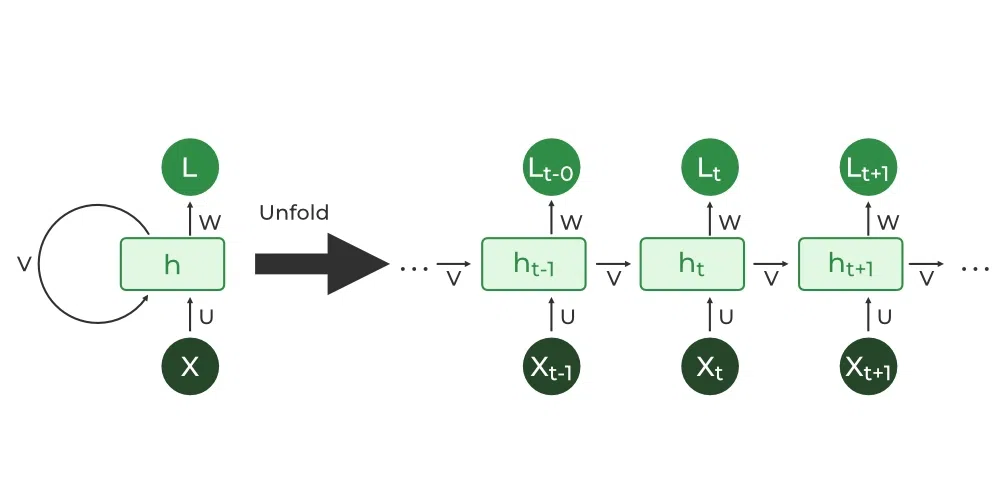
\includegraphics[scale=0.4]{img/rnn_1.png}
          \end{center}
          \textbf{Input units:} At time-step $t$, a RNN takes as input $\vx_t$,
          which is a representation of the $t$-th element of a given sequence,
          e.g.\ a word embedding.
          It then transforms it via matrix $\mU$, and passes this transformed
          input to hidden state $\vh_t$.

          \textbf{Hidden units:} In addition to the transformed input $\vx_t$, a
          hidden state $\vh_t$ takes as additional input $\vh_{t-1}$, i.e.\ the
          hidden state at previous time-step $t-1$, but transformed by matrix
          $\mV$.
          This connection between the same hidden state across time-steps is the
          recurrent connection that gives the network its name (which comes from
          \href{https://en.wikipedia.org/wiki/Recurrence_relation}{\underline{recurrent functions}}).
          Thus, $\vh_{t}$ takes as input $\mU\vx_t$ and $\mV\vh_{t-1}$, combines
          them via some operation (usually addition), and then applies a
          (possibly non-linear) activation function $f$, before passing this
          result to the hidden state in time-step $t+1$, i.e.\ $\vh_{t+1}$.
          In other words, $\vh_t = f(\mU\vx_t + \mV\vh_{t-1})$.
          By sharing parameters $\mU,\mV$ and passing hidden state $\vh_i$
          forward, the intuition is that, at any given time-step $t$, $\vh_{t}$
          encodes what the model has ``seen'' in the sequence so far, i.e.\ all
          elements up until $t$.

          \textbf{Output units:} Optionally, the hidden state may also be passed
          to an output unit $\mL_t$, but transformed via some matrix $\mW$ and
          a (potentially non-linear) activation function $g$.
          That is, $\mL_t = g(\mW\vh_t)$.
          Whether we have an output unit per time-step or not depends on the
          task at hand (more in the next question).

          RNNs are different from FNNs in that they share parameters across
          time-steps, and are thus deep in time.
          This is different from fully-connected networks in that those
          typically use different weight matrices in each hidden layer.
          However, RNNs can also be stacked to become deep in the same sense as
          fully-connected neural networks.
          That is, an RNN layer may produce an output for each input element,
          thus producing an output sequence, which can in turn be used as input
          for another RNN layer.
          In such cases, parameters are not shared across layers.
    \item In \emph{sequence classification}, we require a single prediction per
          sequence. E.g.\ in sentiment classification, we may predict whether a
          given sentence describes a positive or negative sentiment, i.e.\
          binary classification.
          Thus, we do not need an output unit per element in the input unit.
          Instead, we may produce a single output input based on the hidden
          state of the final time-step.
          This output may be passed by a softmax function that produces a
          probability vector of as many components as there are target classes,
          or in the case of binary classification, a logistic function.
          The following figure illustrates such an architecture.
          \begin{center}
              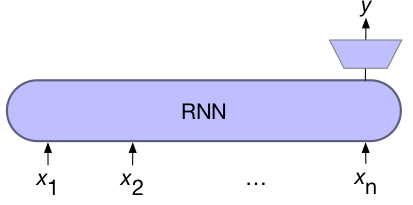
\includegraphics[scale=0.5]{img/sequence_classification_1.png}
          \end{center}

          Conversely, requiring a label for each time-step is known as
          \emph{sequence labeling}.
          For example, in POS tagging, we want to determine whether each word in
          a sentence is a verb, noun, etc.
          Here, the RNN should produce an output at each time-step, as
          illustrated by the image below.
          \begin{center}
              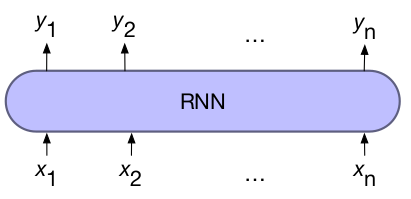
\includegraphics[scale=0.5]{img/sequence_labeling_1.png}
          \end{center}
          Each output unit could include a softmax function for classification.

          In both cases, the inputs and hidden states are as described in answer
          to question (a) above.
    \item Language models predict the next word given a sequence of $n$ previous
          words.
          This is done by producing an output at each time-step given the
          corresponding input element and the hidden state at the previous
          time-step.
          Thus, unlike LMs implememented with fully-connected networks, such as
          the model from Bengio et al. (2003), here we do not have a maximum
          length of the input sequence that we accept, but can take arbitrarily
          long input sequence.
          In addition, unlike n-gram models, predictions made by RNN-based
          language models are not limited by any fixed number of previous words,
          since the hidden state can \emph{in principle} encode all the sequence
          seen so far.
    \item Bidirectional RNNs use an additional hidden state to process a given
          sequence from right to left.
          These hidden states are passed ``backward'' from the end of the
          sequence to the beginning, thus encoding it in the opposite direction.
          This allows the model to, at time-step $t$, encode information about
          both previous and subsequent elements in the input sequence.
          Thus, the model has more context to make predictions at any given
          time-step.
          A disadvantage is that this is more costly to train, and more
          importantly, such a model cannot be used to make real-time
          predictions, since we do not have information about future time-steps.

          Perhaps more importantly, isn't it \emph{cheating} to use information
          about future time-steps?
          Well, that depends on the application.
          If the information is available at inference time, then why not use
          it?
          For example, in machine translation, we are usually given an entire
          sequence to translate, so a model can be trained to read the entire
          sequence in both directions before producing a sequence in the target
          language.
          This intuition extends to the information we give to any model during
          training, independent of its architecture.
          For example, when the goal is to learn generally useful word
          representations, then why not use information in both directions to
          make better use of the context of words in the training set?
          This is what the transformer-based model BERT does.
          Conversely, when predicting the next word in a sequence, models
          typically have access only to previous words.
          Thus, it would not make sense to train models to use information
          about future time-steps to make predictions, as this information is
          not available at inference time.
    \item The main problem with RNN-based models is that the hiddens state needs
          to encode the entirety of a sequence.
          In practice, it's often the case the the hidden states ``remembers''
          information mostly aobut the most recently seen elements, and not
          those seen far into the past.
          This is mostly due to the vanishing gradient problem, which describes
          the impact that operators have over gradient information over a long
          period of time.
          Specifically, if an operator makes a gradient smaller, applying the
          same operator multiple times would continuously reduce this gradient.

          LSTM units were designed to address this issue by allowing the model
          to control what to remember and what to forget about the information
          it has seen.
          This allows a model to realize during training that, in order to
          reduce the loss, it's more convenient to retain some information
          further in the past instead of using more recently seen information.
          This is not possible in vanilla RNNs.

          LSTM units use parameterized gated mechanisms to allow the model to
          control the flow of information across time-steps. Specifically, it
          uses the following gates:
          \begin{itemize}
              \item \textbf{Forget Gate:} allows model to delete information
                    that it has seen but no longer needs.
              \item \textbf{Input/Add Gate:} allows model to select what
                    information from the current input and hidden state to use.
              \item \textbf{Output Gate:} allows the model to separate
                    information needed to produce current output from what is
                    needed to pass to future time-steps.
          \end{itemize}
    \item An encoder-decoder architecture is made up of three components: an
          encoder which takes as input a given source sequence, a context vector
          produced by the encoder that represents the input sequence, and a
          decoder, which takes as input the context vector and produces an
          output sequence.
          Let's describe the encoder and decoder in more detail.

          \textbf{Encoder:} In machine translation, the encoder takes as input
          the source sequence, and produces a context vector (usually the
          hidden state of the last time-step).
          This encoder produces no other outputs and general can be any
          architecture that makes as much use of the input data as possible.
          RNN-based encoders are typically stacked bidirectional RNNs with LSTM
          units (biLSTMs for short), but this can also be done with other types
          of architectures, e.g.\ transformers.

          \textbf{Decoder:} The decoder takes as input the context vector and a
          a ``beginning of sentence'' tag (in machine translation, this tag is
          used to separate source from target sentences pairs shown to the
          model).
          Using this, it produces a hidden state and an output word,
          \emph{both of which} are then used as input for the hidden state of
          the decoder in the next time step.
          In addition, it's common to use the context vector produce by the
          encoder as input in each time-step of the decoder, to preserve this
          information.
          Formally, the hidden state of the decoder at time-step $t$ is given
          by:
          \begin{align*}
              \vh_t^d & = g(\vy_{t-1},\vh_{t-1}^d,\vc),
          \end{align*}
          where $\vy_{t-1}$ is the embedding of word produce by decoder in the
          previous time-step, and $\vc$ is the context vector produced by the
          encoder.
          This decoder architecture is illustrated in the image below.
          \begin{center}
              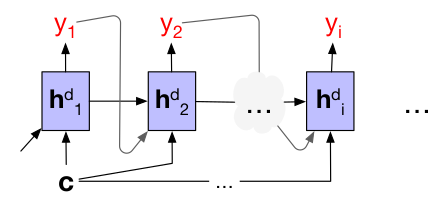
\includegraphics[scale=0.5]{img/encoder_decoder_for_mt_1.png}
          \end{center}
\end{enumerate}

\section{Sampling for Text Generation}

\begin{enumerate}[label=(\alph*)]
    \item
          \begin{enumerate}[label=(\roman*)]
              \item \textbf{Autoregressive generation:} generate sequence of
                    word/tokens by repeatedly sampling the next word/token
                    conditioned on previously chosen words/tokens.
              \item \textbf{Advantages:} can capture dependencies between
                    words/tokens in a sequence.
              \item \textbf{Disadvantages:} can be slow to generate long
                    sequences, then longer the range of dependencies that need
                    to be captured, the higher the cost of sampling.
                    In other words, non-autoregressive generation is
                    cheaper/faster.
          \end{enumerate}
    \item $p(y_t|y_{<t},X,\theta)$
    \item
          \begin{algorithmic}
              %   \STATE $i \leftarrow 1$
              \STATE $w \leftarrow \operatorname{sample}(p(w_i|<s>))$
              \STATE out $\leftarrow [w]$
              \WHILE{$w \neq </s>$}
              %   \STATE $i \leftarrow i + 1$
              \STATE $w \leftarrow \operatorname{sample}(p(w_i|out))$
              \STATE out $\leftarrow$ out $+ [w]$
              \ENDWHILE
              \RETURN out
          \end{algorithmic}

    \item Advantages are that it is straightforward to understand and implement.
          But an important disadvantage is that it can lead to generation of
          text that is predictable and repetitive.
          In fact, given a model and the same input sequence, greedy sampling
          should deterministically produce the same output sequence.
          This is convenient when we want to predict facts that do not change,
          e.g.\ the answer to ``What is the capital of Germany''?
          But this is an undesired property when we want to generate text that
          is more original/creative, such as what should follow after ``The
          title of my talk is''
    \item Random sampling can lead to more diverse and creative text, as it
          allows the model to sample from the entire vocabulary.
          However, it can also lead to less coherent text, as the model may
          sample words that are less likely to follow the previous words.
          In addition, the size of the vocabulary is often very large, and for
          a given input sequence, the distribution over words is very skewed.
          This means that the model may sample from words that are very rare,
          and thus produce text that is less coherent.
    \item The answer is \emph{top-k} sampling. This is a generalization of
          \emph{greedy} sampling, where we now sample from the set of $k$ words
          with the most probability.
          When $k=1$, we have greedy sampling, and when $k=|V|$, we have random
          sampling.
          Generally, for values of $k > 1$, we allow the model to generate words
          that are not so predictible, but still probable enough that the
          resulting text can be of high-quality.

          One important disadvantage of \emph{top-k} sampling is that $k$ is a
          fixed value, but the distributions over words produced by a model
          change for given inputs.
          E.g.\ when the input sequence is ``The capital of Germany is'', most
          of the probability mass in the resulting distribution would ideally be
          in the Berlin token (or combination of tokens), which is a (proper)
          noun.
          But when the input sequence is ``The title of my talk'', the
          probability mass would most likely be in the token ``is'' or similar
          verbs.
          To address this issue, \emph{top-p} sampling was proposed, where we
          sample from the words that add up to the top $p$ probability mass in
          the distribution. That way, we can sample from a variable number of
          words given different input sequences.
          A good model may indeed learn to put most of the mass in the answer to
          a factual question, e.g. Berlin is the capital of Germany, or more
          generally distribute it more evenly among several probable words in
          other settings.
    \item As $tau$ approaches zero and is less than 1, it will increase the
          values of all logits, e.g.\ $12 < 12/0.5 < 12/0.3$.
          This will result in increased probability mass on words that already
          have high mass, and decreased probability mass on words that had low
          mass in the first place.
          Thus, as we decrease the temperature, most of the probability mass in
          the distribution concentrates around the most probable words.
          Conversely, if we increase the temperature to values greater than 1
          and beyond, the probability mass will be more evenly distributed
          across all words, as the operation will decrease values of all logits.
          See some animations
          \href{https://medium.com/@harshit158/softmax-temperature-5492e4007f71}{\textcolor{blue}{\underline{here}}}.
\end{enumerate}


\end{document}
